\documentclass[conference]{IEEEtran}
\usepackage{cite}
\usepackage{amsmath,amssymb,amsfonts}
\usepackage{graphicx}
\usepackage{tabularx}
\usepackage{multirow}
\graphicspath{{figures/}}
\usepackage{textcomp}
\usepackage{xcolor}
\def\BibTeX{{\rm B\kern-.05em{\sc i\kern-.025em b}\kern-.08em
    T\kern-.1667em\lower.7ex\hbox{E}\kern-.125emX}}
\begin{document}

\title{Diseño de sistema distribuido para reserva de eventos \\
    \vspace{1cm}

    \large 
    Richard Manuel Castillo Pesca \\
    Lorenzo Ramírez Calderón \\

    \vspace{1cm}
    Pontificia Universidad Javeriana \\ 
    Introducción Sistemas Distribuidos \\
    Mariela Curiel Huerfano \\ 
    Bogota, Colombia \\
    11 de octubre, 2026
}

\author{}


\maketitle

\begin{abstract}
This document is a model and instructions for \LaTeX.
This and the IEEEtran.cls file define the components of your paper [title, text, heads, etc.]. *CRITICAL: Do Not Use Symbols, Special Characters, Footnotes, 
or Math in Paper Title or Abstract.
\end{abstract}


\section{Introducción}


\section{Modelos del sistema}

\subsection{Arquitectonico}
El sistema implementa un modelo arquitectónico por capas, contando con un total de 3 capas. La primera capa
es la capa de consumidores donde los procesos clientes solicitan transacciones al gestor de transacciones que 
pueden ser reservas de asientos, modificaciones de reserva, consulta de eventos en un determinado mes o cancelaciones
de reserva.

La segunda capa es la capa de servicios de negocio donde se encuentra el gestor de transacciones encargado de
recibir las solicitudes de los clientes y decidir el servicio de procesamiento y canal que se utilizara para la solicitud.
Las peticiones serán dirigidas por el canal síncrono si se tratan de reservas, consultas o modificaciones, o por el canal 
asíncrono si es una petición de cancelación. Las peticiones síncronas son procesadas por el servicio de procesamiento
de reservas/modificaciones/consultas  (RMC), mientras que las peticiones asíncronas son procesadas por el servicio de 
cancelaciones y notificaciones.

La tercera y última capa es la capa de servicios de almacenamiento que se encarga del manejo de transacciones sobre
la base de datos principal al recibir solicitudes de escritura y lectura de ambos servicios de procesamiento.

\subsection{Interacción}

El sistema es un sistema distribuido asincrónico debido a que no hay limitaciones en los tiempos de ejecución de
procesos del sistema ni en los retardos en transmisión de mensajes. Del mismo modo, no se asumen límites conocidos en las tasas de deriva
de los relojes locales de cada proceso. Esta decisión refleja la naturaleza inherentemente impredecible de la red y los sistemas
distribuidos, esto permite que el diseño posea una mejor tolerancia a fallos y escalabilidad al no depender de restricciones
temporales estrictas en los componentes.

La interacción en relación con el envío de mensajes utiliza mecanismos de comunicación acoplados y desacoplados en el
tiempo e inicialmente acoplados en el espacio. Este modelo de comunicación permite cumplir con los requerimientos del
sistema en cuanto a las solicitudes de cancelación las cuales deben ser asíncronas (no bloqueantes) y el
resto de transacciones de reserva de eventos las cuales son síncronas al esperar la confirmación de las capas subsecuentes.
La arquitectura inicial es acoplada en el espacio dado que los servicios se encuentran direccionados directamente y cada uno
cuenta con una sola réplica. Este acoplamiento temporal será reducido posteriormente al considerar componentes de
escalabilidad y tolerancia a fallos, puesto que las solicitudes serán distribuidas a través de diferentes instancias de los servicios.


\subsection{Fallos}

El modelo de fallos contempla tanto fallos en la red como en cada uno de los procesos del sistema. Al ser un sistema
con un modelo de interacción asincrónico, no existen límites superiores conocidos para el tiempo de ejecución de procesos
o envió y recepción de mensaje. Por lo anterior no se consideran fallos de prestaciones, ya que no existe límites
para determinar si una respuesta está fuera de los tiempos esperados. De igual forma, no se asume fallos tipo
Fail/Stop, puesto que la inexistencia de límites temporales hace que no se pueda
determinar con certeza si un proceso ha fallado o se ha ejecutado con retraso.

Por lo anterior el sistema considera principalmente fallos de ruptura y omisión.
Los fallos de ruptura corresponden a situaciones en las que un proceso como el Gestor de Transacciones pueden fallar.
Por otro lado, los fallos de omisión contemplan situaciones en las que un mensaje no es enviado, se pierde durante la
comunicación o no es recibido por su destinatario.

Finalmente, los componentes del sistema se consideran libres de fallos bizantinos es decir que al fallar dejan de operar
en vez de producir y enviar información arbitraria.

\subsection{Seguridad}


\section{Diseño del sistema}

El diseño del sistema refleja la arquitectura base planteada. Este cumple con los requerimientos
de despliegue físico y separación de responsabilidades permitiendo las diferentes interacciones que 
los clientes pueden tener con el servidor.

\subsection{Despliegue}

El diagrama de despliegue (Fig. \ref{DiagramaDespliegue}) expone la distribución física del sistema a través de tres máquinas distintas cada
una siendo una capa de la arquitectura del sistema. De este diagrama se debe destacar los protocolos de comunicación
seleccionados teniendo en cuenta el modelo de comunicacion sincrónico y asincrónico del sistema. Para ello se utiliza el protocolo
sincrónico REQ/REP de ZeroMQ para todo el flujo de solicitudes sincrónicas. En el caso de cancelación el cual debe
ser asincrónico para el cliente se manejan distintos protocolos teniendo en cuenta los requerimientos de comunicación
entre servicios. Para ello se usa
el patrón Router/Dealer para las notificaciones al cliente una vez hecha la cancelación y el llamado al gestor de transacciones al
cliente. Ademas se usa el patron Pull/Push para los llamados al servicio de cancelación por su comunicación unidireccional
y división de tareas considerando las modificaciones a futuro para la escalabilidad del sistema.


\begin{figure}[htbp]
    \centerline{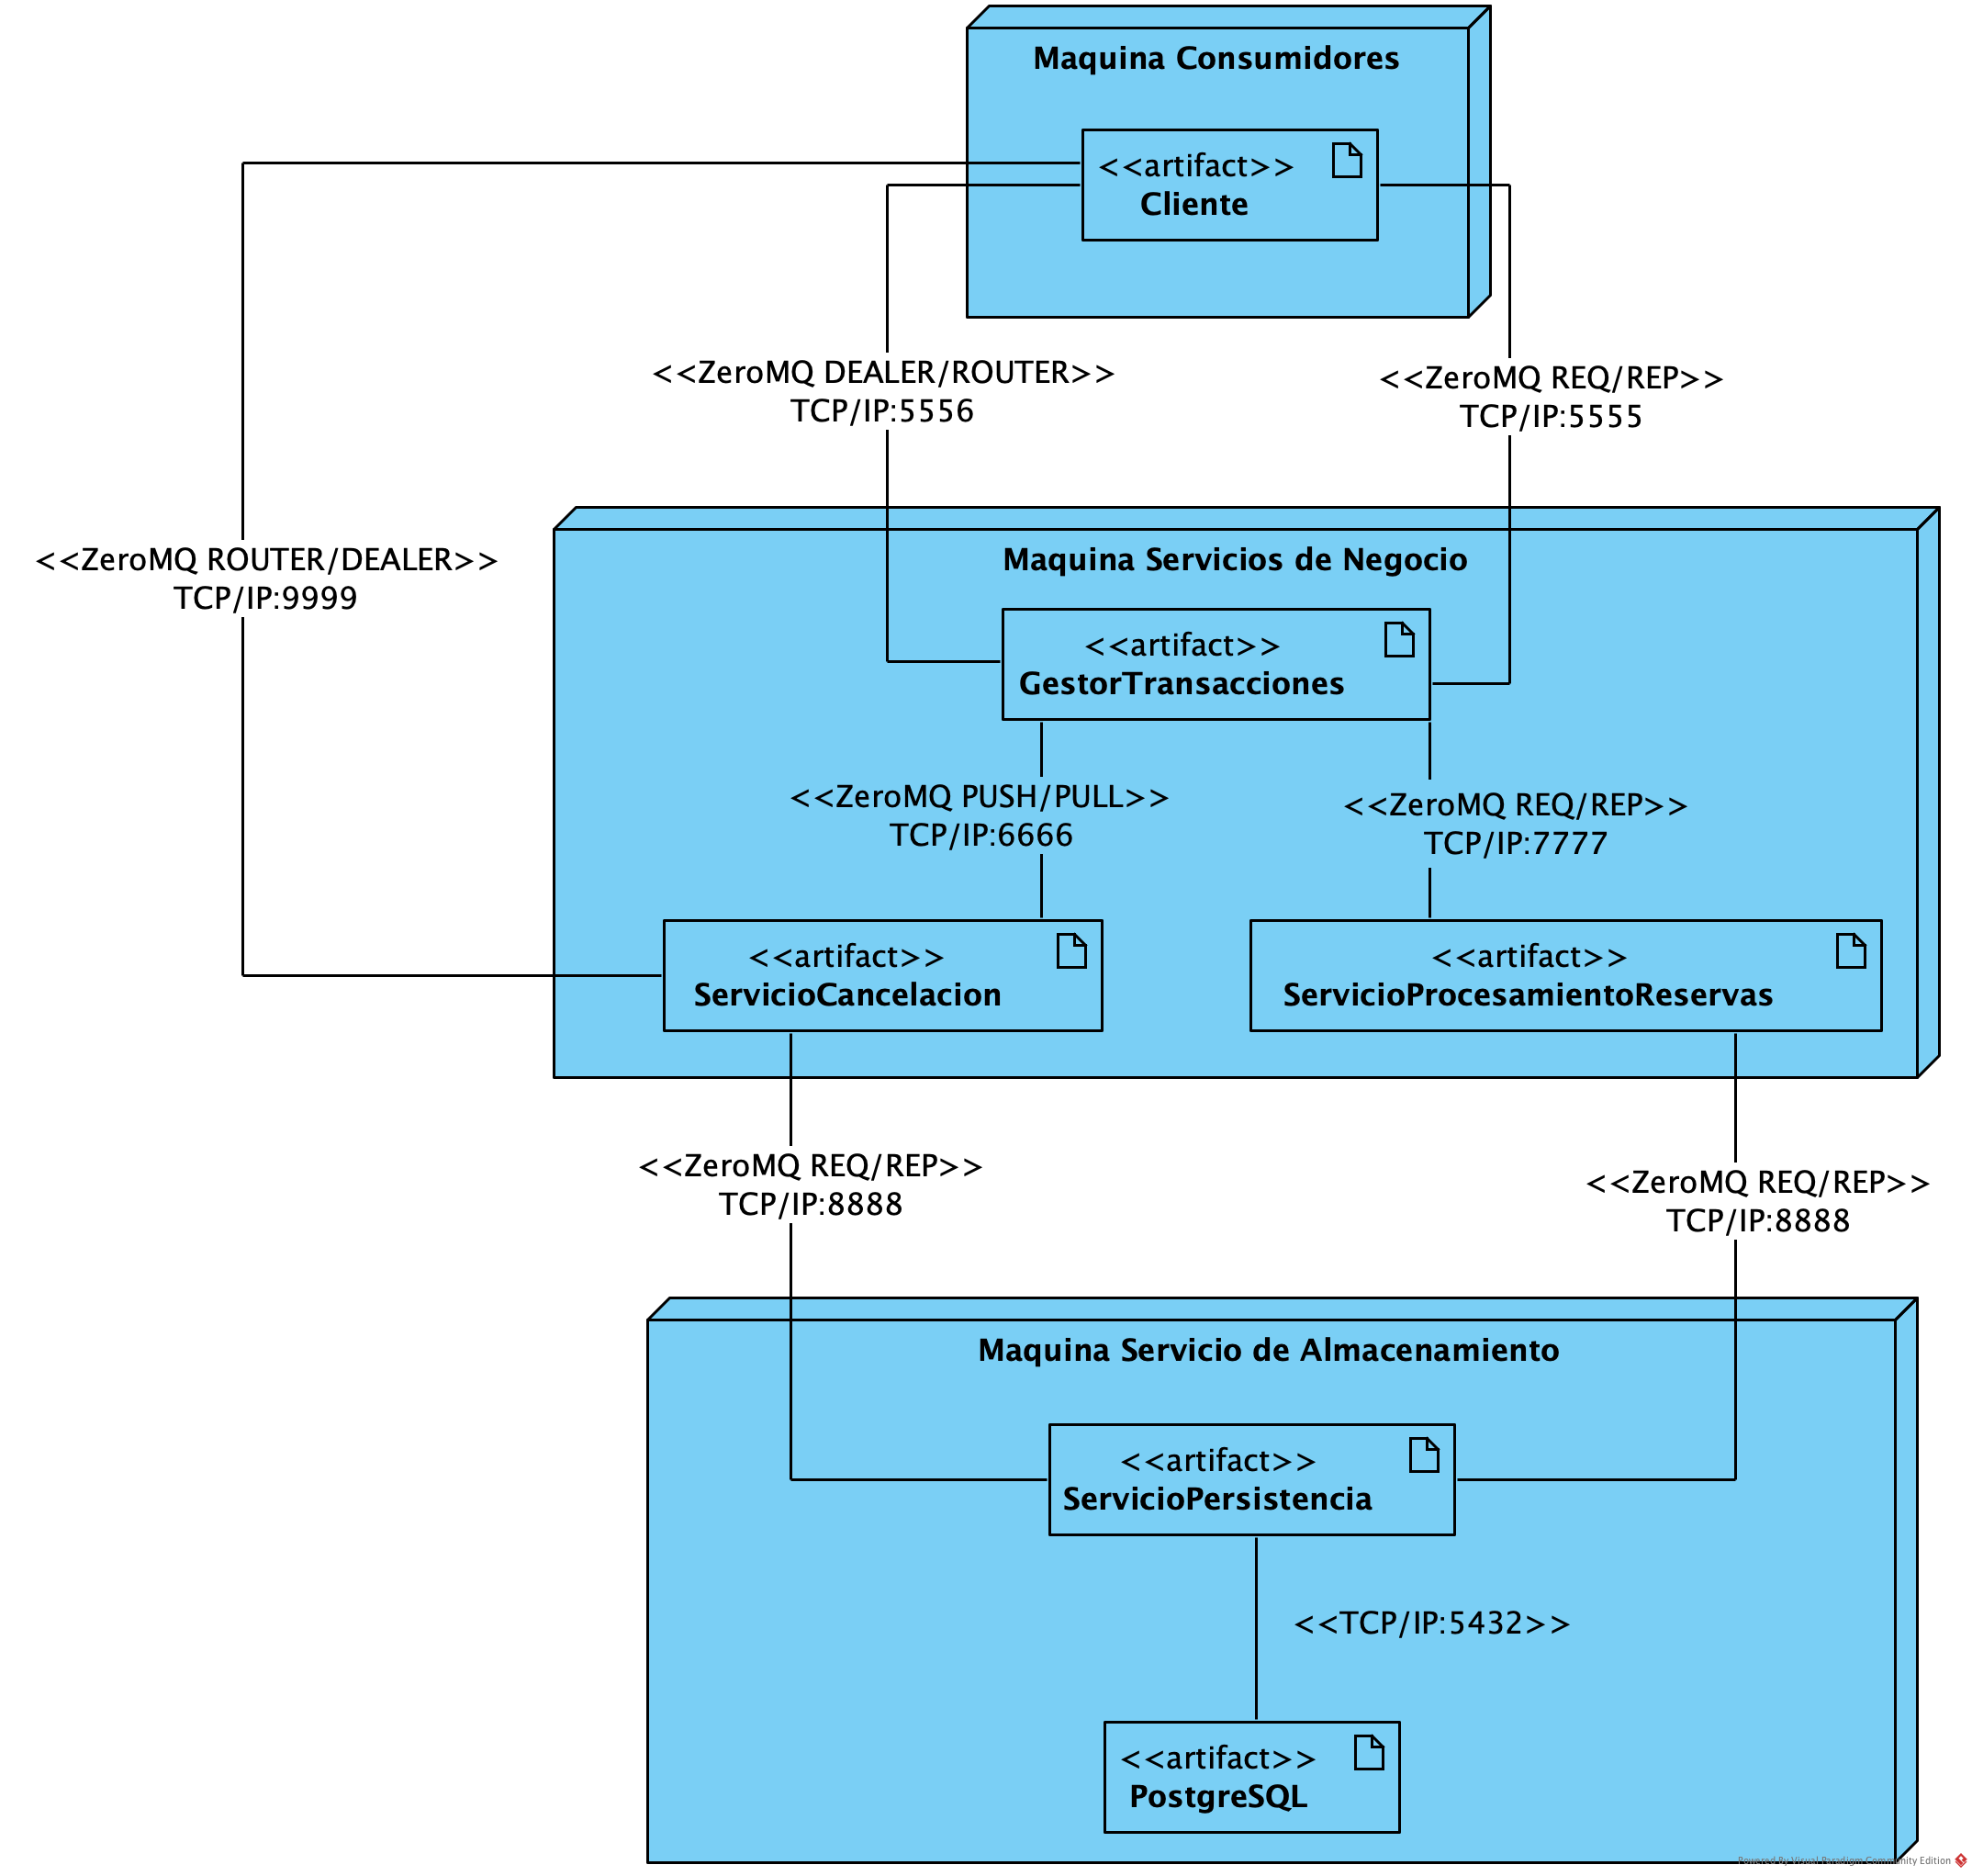
\includegraphics[width=\columnwidth]{despliegue.png}}
    \caption{Diagrama de despliegue.}
    \label{DiagramaDespliegue}
\end{figure}


\subsection{Componentes}

El diagrama de componentes (Fig. \ref{DiagramaComponentes}), expone la distribucion logica del sistema de reserva. 
En esta se evidencia las interfaces que expone cada uno de los componentes del sistema y sus respectivos consumidores.
Estas siguen el flujo logico de los requerimientos del sistema, donde el cliente envia solicitudes al Gestor de Transacciones, 
el cual redirige las las operaciones al Servicio de Cancelacion o RMC dependiendo del tipo de solicitud. 
Ambos servicios utilizan la interfaz del servicio de persistencia para acceder a la informacion alamacenada de los eventos. 
Finalmente, se evidencia la interfaz de notificacion expuesta por el cliente, la cual el servicio de cancelacion utiliza
para enviar notificaciones de forma asincronica. 

La definición de los métodos correspondientes a cada una de las interfaces se presenta en el diagrama de 
clases del sistema, donde se detallan las operaciones que ofrece cada interfaz y su respectiva implementación.

\begin{figure}[htbp]
    \centerline{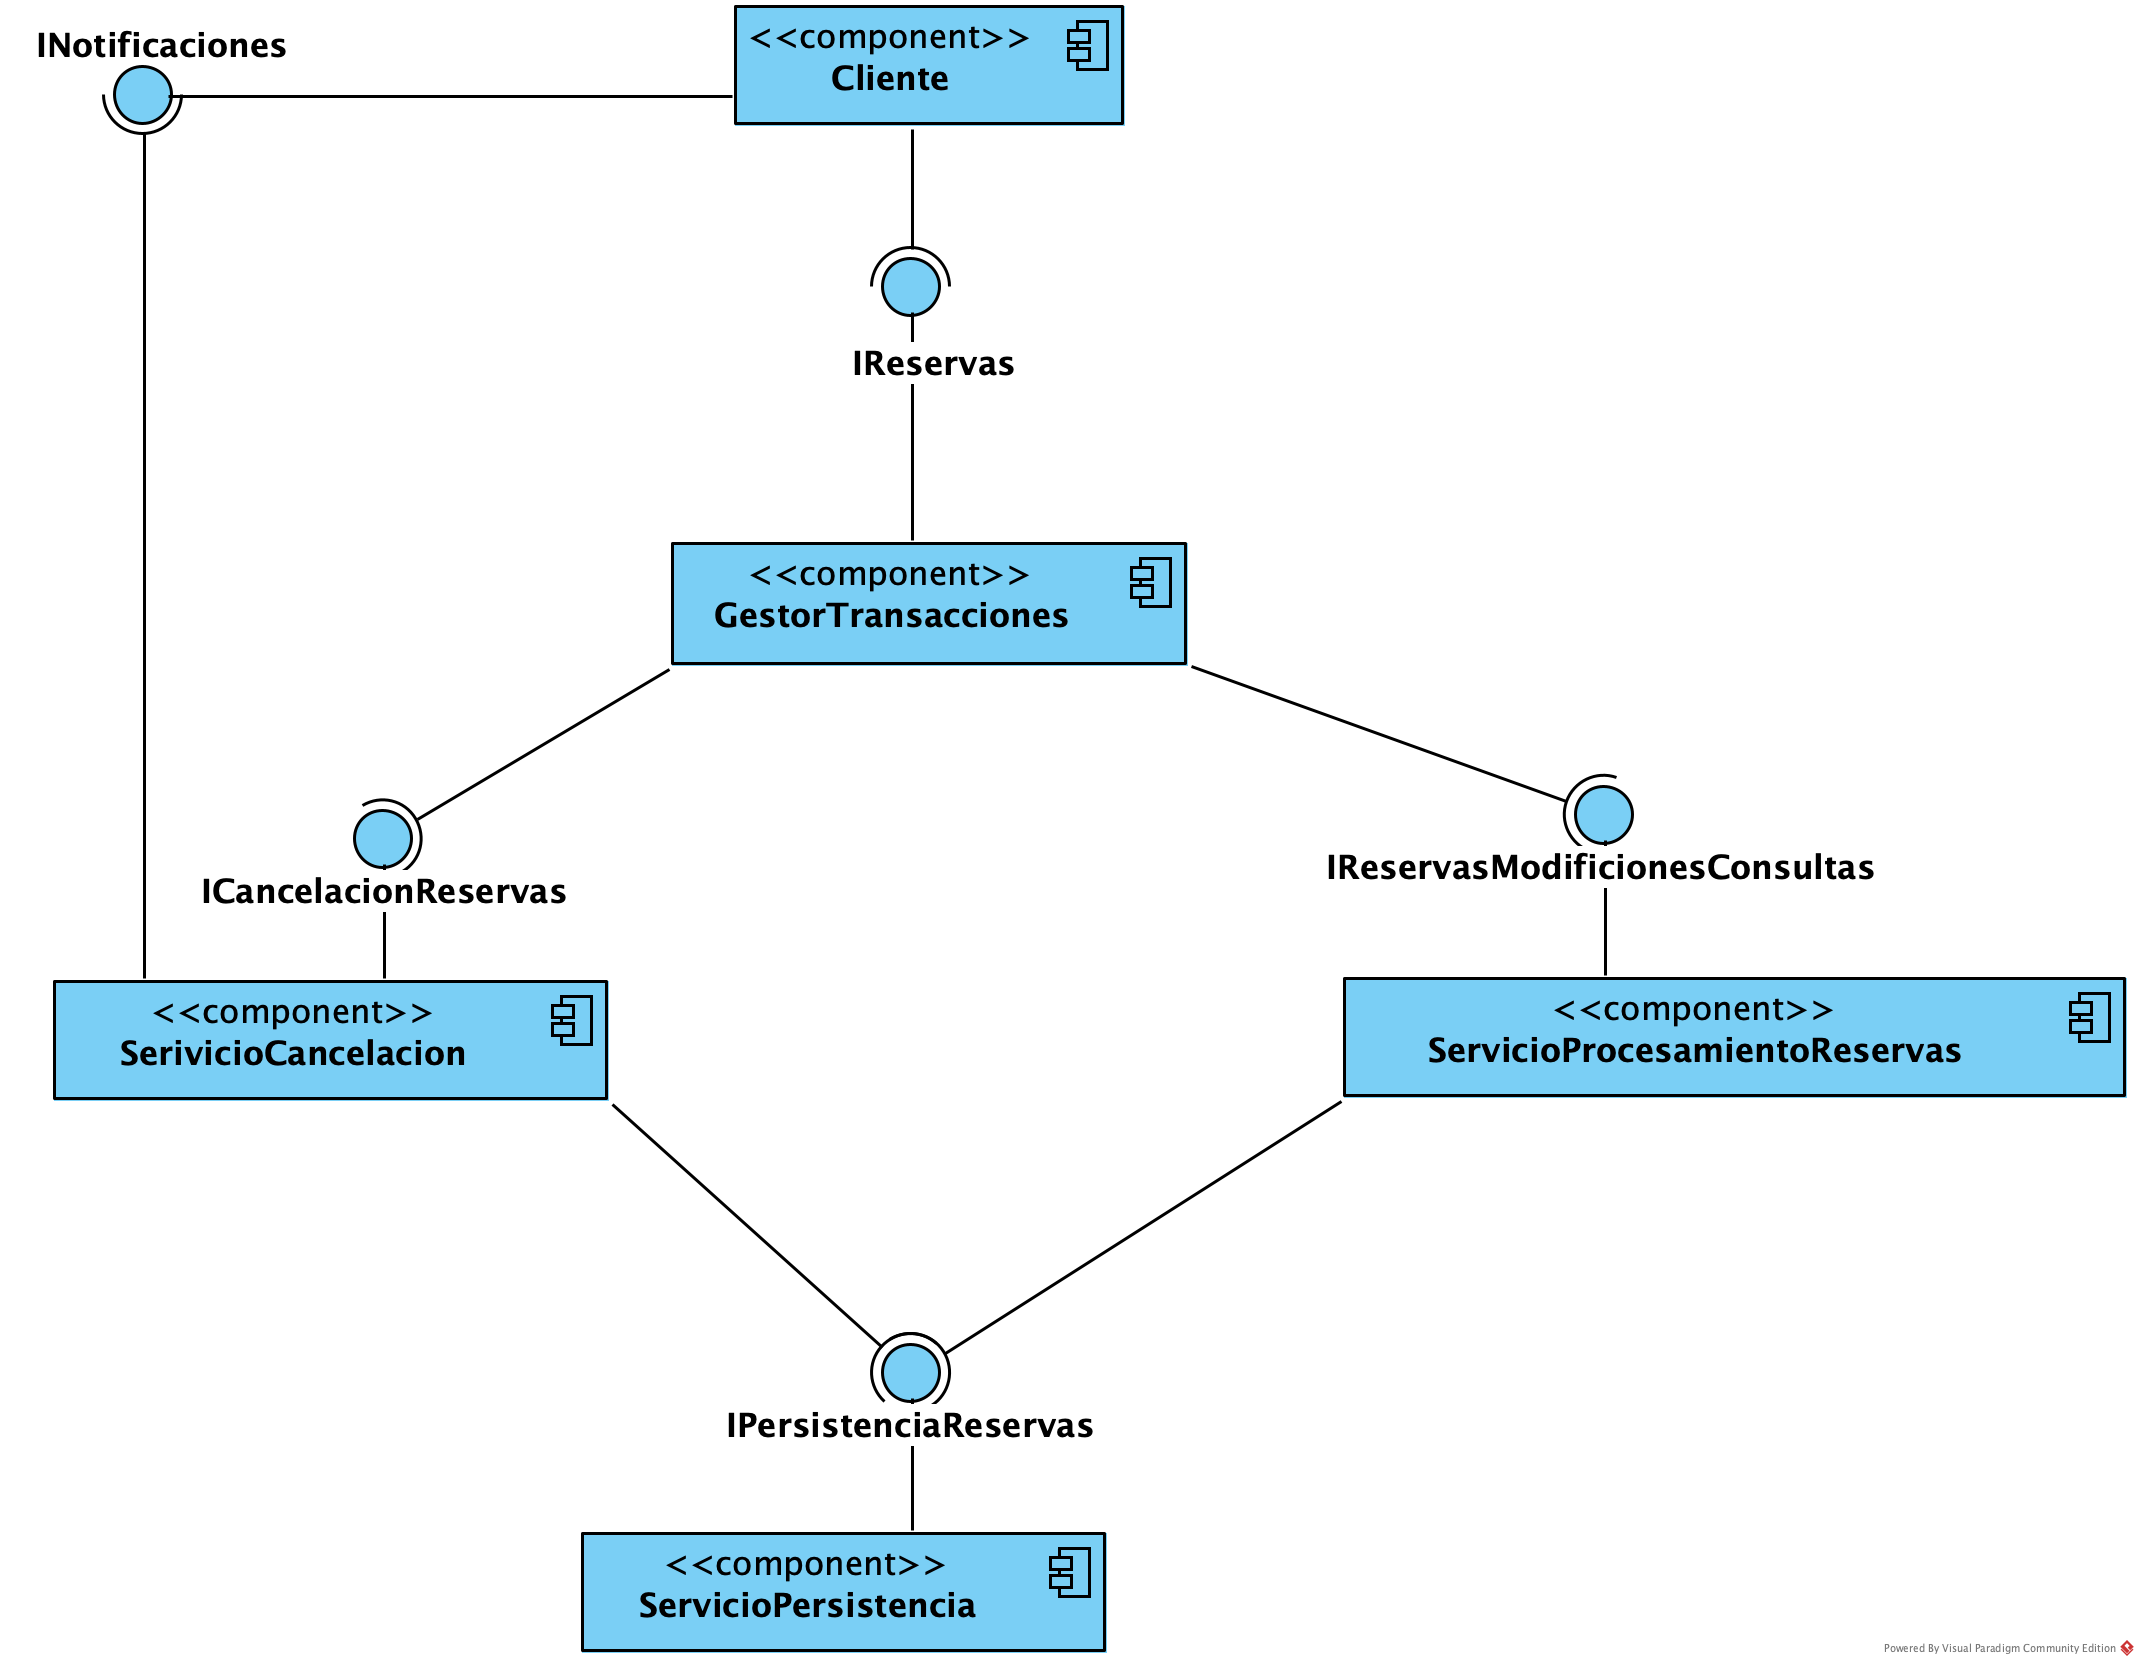
\includegraphics[width=\columnwidth]{componentes.png}}
    \caption{Diagrama de componentes.}
    \label{DiagramaComponentes}
\end{figure}

\subsection{Clases}

\subsection{Secuencia}

\section{Escalabilidad y tolerancia a fallos}

La escalabilidad y tolerancia a fallos sera llevada a cabo 



\section{Protocolo de pruebas}

El protocolo de pruebas del sistema contempla diferentes niveles de validacion para asegurar su correcto
funcionamiento y posterior medicion de rendimiento ante diferentes cargas y tolerancia a fallos.

Primeramente se realizaran pruebas unitarias sobre la logica de los diferentes servicios




En relacion a las pruebas del sistema distribuido se realizaran pruebas concurrentes con diferentes numeros de clientes 
que realicen operaciones simultaneamente. De esta manera se evaluara el comportamiento y rendimiento
del sistema ante diferentes cargas de operaciones. Como se muestra en la Tabla \ref{tab:pruebas_rendimiento} 
se obtendran metricas que evaluen y comparen el diseño de la arquitectura base y la arquitectura escalable 
propuesta en la seccion anterior. Cada prueba de carga contempla una generacion de operaciones por parte de los clientes 
de 3 minutos.

Asimismo se considerara una prueba de fallo y resilencia mediante la interrupcion voluntaria del Gestor de Transacciones.
Ante esta falla se espera que el sistema instancie un nuevo proceso que sustituya al servicio.
En esta prueba se evaluara que el servicio pueda retomar la operacion del sistema, siendo esta falla transparente para el cliente
al poder retomar las operaciones desde la interrupcion.


\begin{table}[htpb]
\centering
\caption{Pruebas de rendimiento}
\label{tab:pruebas_rendimiento}
\begin{tabularx}{\columnwidth}{|X|X|}
\hline
\textbf{Carga} & \textbf{Métricas} \\ \hline

3 clientes: 2 consultas y 1 consulta con reserva
&
\multirow{3}{\linewidth}{%
Tiempo promedio y desviación estándar de consultas y reservas. 
Transacciones por minuto de consultas y reservas.
}
\\ \cline{1-1}

5 clientes: 3 consultas y 2 reservas y modificaciones.
&
\\ \cline{1-1}

8 clientes: 4 consultas y 4 reservas y modificaciones.
&
\\ \hline

\end{tabularx}
\end{table}

\section{Estrategias de obtencion de metricas}
Para obtener las metricas de desempeño se utilizara un generador de carga, Python y la libreria \texttt{pandas}.
Estas seran hechas en el Cliente y el Gestor de Transacciones.

Para consultas y reservas se medira el tiempo de respuesta de cada solicitud en el cliente con \texttt{time.perf\_counter}, 
tomando como inicio el envio de la solicitud al Gestor de Transacciones hasta que recibe su respectiva respuesta.
Cada medicion sera almacenada en un archivo junto con el tipo de operación.
Posteriorimente mediante \texttt{pandas} se calculara el promedio y la desviación estándar de cada tipo de operacion.

Para las transacciones por minuto (TPM) se el Gestor de Transacciones registrara cada 
solicitud atendida junto a su marca de tiempo y tipo de operación en un archivo. A partir de los registros
se cuantifican las transacciones procesadas de cada tipo durante el periodo de medicion definidio en el plan de pruebas de 3 minutos,
calculando finalmente la tasa de transacciones por minutuo.

\section{Generacion de carga clientes}
\section{Generación de carga}
La carga se genera con Locust usando un usuario personalizado en Python que se comunica con el Gestor de Transacciones mediante pyzmq, 
cada cliente tiene su propio socket REQ y construye cada mensaje con el mismo formato del struct Request.

Los clientes toman sus datos de un archivo load_data.json, generado con un script que crea identificadores de cliente, eventos, 
meses y ocurrencias. La base de datos se carga a partir de ese mismo archivo, de modo que los identificadores coinciden en ambos lados. 

En cada solicitud, el cliente elige de forma aleatoria (utilizando la función random.choice de la librería random) el mes en el caso de
la consulta y el evento, la ocurrencia y el número de asientos en el caso de la reserva. Por lo anterior, se cuenta con dos tipos de 
cliente: uno que solo consulta y otro que consulta y reserva, lo que permite simular los escenarios de la Tabla 1.


\section{Introduction}
This document is a model and instructions for \LaTeX.
Please observe the conference page limits. 


\subsection{Abbreviations and Acronyms}
Define abbreviations and acronyms the first time they are used in the text, 
even after they have been defined in the abstract. Abbreviations such as 
IEEE, SI, MKS, CGS, ac, dc, and rms do not have to be defined. Do not use 
abbreviations in the title or heads unless they are unavoidable.

\subsection{Some Common Mistakes}
\begin{itemize}
\item The word ``data'' is plural, not singular.
\item The subscript f ``i.e.'' means ``that is'', and the abbreviation ``e.g.'' means ``for example''.
\end{itemize}



\subsection{Figures and Tables}
\paragraph{Positioning Figures and Tables} Place figures and tables at the top and 
bottom of columns. Avoid placing them in the middle of columns. Large 
figures and tables may span across both columns. Figure captions should be 
below the figures; table heads should appear above the tables. Insert 
figures and tables after they are cited in the text. Use the abbreviation 
``Fig.~\ref{fig}'', even at the beginning of a sentence.

\begin{table}[htbp]
\caption{Table Type Styles}
\begin{center}
\begin{tabular}{|c|c|c|c|}
\hline
\textbf{Table}&\multicolumn{3}{|c|}{\textbf{Table Column Head}} \\
\cline{2-4} 
\textbf{Head} & \textbf{\textit{Table column subhead}}& \textbf{\textit{Subhead}}& \textbf{\textit{Subhead}} \\
\hline
copy& More table copy$^{\mathrm{a}}$& &  \\
\hline
\multicolumn{4}{l}{$^{\mathrm{a}}$Sample of a Table footnote.}
\end{tabular}
\label{tab1}
\end{center}
\end{table}

\begin{figure}[htbp]
\centerline{
\includegraphics{fig1.png}}
\caption{Example of a figure caption.}
\label{fig}
\end{figure}

Figure Labels: Use 8 point Times New Roman for Figure labels. Use words 
rather than symbols or abbreviations when writing Figure axis labels to 
avoid confusing the reader. As an example, write the quantity 
``Magnetization'', or ``Magnetization, M'', not just ``M''. If including 
units in the label, present them within parentheses. Do not label axes only 
with units. In the example, write ``Magnetization (A/m)'' or ``Magnetization 
\{A[m(1)]\}'', not just ``A/m''. Do not label axes with a ratio of 
quantities and units. For example, write ``Temperature (K)'', not 
``Temperature/K''.


\section*{References}

Please number citations consecutively within brackets \cite{b1}. The 
sentence punctuation follows the bracket \cite{b2}. 


\begin{thebibliography}{00}
\bibitem{b1} G. Eason, B. Noble, and I. N. Sneddon, ``On certain integrals of Lipschitz-Hankel type involving products of Bessel functions,'' Phil. Trans. Roy. Soc. London, vol. A247, pp. 529--551, April 1955.
\bibitem{b2} J. Clerk Maxwell, A Treatise on Electricity and Magnetism, 3rd ed., vol. 2. Oxford: Clarendon, 1892, pp.68--73.

\end{thebibliography}

\end{document}

